% 10 pages, excluding references
% Abstract 05/12
% Paper 12/12
% CCGrid will be following a double-blind review process
% IEEE two-column conference proceedings template

\documentclass[conference,10pt]{IEEEtran}

\def\BibTeX{{\rm B\kern-.05em{\sc i\kern-.025em b}\kern-.08em
    T\kern-.1667em\lower.7ex\hbox{E}\kern-.125emX}}

\usepackage[utf8]{inputenc}
\usepackage{amsmath, amssymb, amsfonts, colortbl, xspace, todonotes, paralist, multirow, hyperref, pgfplots}
\pgfplotsset{compat=newest}
\hypersetup{
   colorlinks=false,
   pdfborder={0 0 0},
}
\usepackage[english]{babel}
\usepackage{graphicx, color, amssymb, url, xcolor, tikz, pgf, float, subcaption, algorithm,  tabularx}
\usepackage[noend]{algpseudocode}
\usetikzlibrary{trees, shapes, calc, external, fit, arrows, decorations, decorations.pathreplacing, patterns, automata, positioning, arrows.meta, intersections, calligraphy}

% Custom commands
\algnewcommand\algorithmicforeach{\textbf{for each}}
\algdef{S}[FOR]{ForEach}[1]{\algorithmicforeach\ #1\ \algorithmicdo}
\renewcommand{\algorithmicrequire}{\textbf{Input:}}
\renewcommand{\algorithmicensure}{\textbf{Output:}}
\newcommand{\Node}[1]{\ensuremath{\mathrm{Node}_{#1}}\xspace}
\newcommand{\flow}[1]{\ensuremath{\mathit{flow}_{#1}}\xspace}
\newcommand{\file}{\ensuremath{\mathit{File}}\xspace}
\newcommand{\storage}{\ensuremath{\mathit{Storage}}\xspace}
\newcommand{\size}{\ensuremath{\mathit{Size}}\xspace}
\newcommand{\memory}{\ensuremath{\mathit{Mem}}\xspace}
\newcommand{\memorymap}{\ensuremath{\mathcal{M}_{map}}\xspace}
\newcommand{\duration}{\mathit{Duration}\xspace}
\newcommand{\bandwidth}{\mathit{BW}\xspace}
\newcommand{\core}{\mathit{Cores}\xspace}
\newcommand{\submissiontime}{\mathit{SubTime}\xspace}
\newcommand{\emptyflow}{\mathit{Reference\_Flow}\xspace}
\newcommand{\Endtime}{\mathit{EndTime}\xspace}
\newcommand{\walltime}{\mathit{WallTime}\xspace}
\newcommand{\completiontime}{\mathit{CompletionTime}\xspace}
\newcommand{\start}{\mathit{StartTime}\xspace}
\newcommand{\allocatednode}{\ensuremath\mathit{\sigma}\xspace}
\newcommand{\allocatedcores}{\ensuremath\mathit{\gamma}\xspace}

\newcommand{\fileset}{\ensuremath{\mathbb{F}}\xspace}
\newcommand{\jobset}{\ensuremath{\mathbb{J}}\xspace}
\newcommand{\nodeset}{\ensuremath{\mathbb{N}}\xspace}
\newcommand{\evict}{\ensuremath{\mathcal{V}}\xspace}
\newcommand{\nbloads}{\ensuremath{\mathit{\mathit{Loads}}}\xspace}
\newcommand{\live}{\ensuremath{L}\xspace}
\renewcommand{\algorithmicrequire}{\textbf{Input:}}
\renewcommand{\algorithmicensure}{\textbf{Output:}}

\begin{document}

\title{Locality-aware batch scheduling of I/O intensive workloads}

\maketitle


\begin{abstract}
  Clusters make use of workload schedulers such as
  the Slurm Workload Manager to allocate computing jobs onto
  nodes. These schedulers usually aim at a good trade-off between
  increasing resource utilization and user satisfaction (decreasing
  job waiting time). However, these schedulers are typically unaware
  of jobs sharing large input files, which may happen in data
  intensive scenarios. The same input files may be loaded several
  times, leading to a waste of resources.
   
  We study how to design a \textit{data-aware job scheduler} that is
  able to keep large input files on the computing nodes, without
  impacting other memory needs, and can use previously loaded files to
  \textit{limit data transfers in order to reduce the waiting times of
    jobs}.

  We present three schedulers capable of distributing the load between
  the computing nodes as well as re-using an input file already loaded
  in the memory of some node as much as possible.
  
  We perform simulations using real cluster usage traces to compare
  them to classical job schedulers.  The results show that
  keeping data in local memory between successive jobs and using data
  locality information to schedule jobs allows a reduction in job
  waiting time and a drastic decrease in the amount of data transfers.


  %%%% Longer version below:
  %   Clusters and supercomputers make use of workload schedulers such as
  % the Slurm Workload Manager or OAR to allocate computing jobs onto nodes. These schedulers
  % usually aim at a good trade-off between increasing resource
  % utilization and user satisfaction (decreasing job waiting
  % time). However, these schedulers are typically unaware of jobs
  % sharing large input files: in data-intensive scenarios, tens to
  % hundreds of jobs dedicated to the study of the same multi-GB input
  % file may be successively submitted. Running each of these jobs
  % first requires to load the input file, leading to a large data
  % transfer overhead. Users could manually group some of these
  % tasks into larger jobs to reduce data transfers, but this would result in less granular units that are
  % more difficult to schedule by the resource manager, and would
  % thus result in a larger delay as well. We study how to design a \textit{data-aware
  %   job scheduler} that is able to keep large input files on the 
  % computing nodes, provided this does not impact the memory needs of
  % other jobs, and can use previously loaded files to \textit{limit
  %   data transfers in order to reduce the waiting times of jobs}.

  % We present three schedulers capable of distributing the load between
  % the computing nodes as well as being aware of what the memory of each
  % node contains in order to re-use an input file
  % already loaded in the memory of some node as many times as possible.
  
  
  % We report simulations performed using real cluster usage traces. 
  % Our approach is compared to currently used schedulers in batch systems.
  % The results show that keeping data locally, in memory, between successive
  % jobs and using data locality information to schedule jobs allows a
  % reduction in job waiting time and a drastic decrease in the amount of data
  % transfers.

  
\end{abstract}

%~ \todo[inline]{LM: I changed memory into storage: is it correct ? Carl: I changed back, the point is that these large files are kept in memory with heavy random accesses. There are of course cases where local scratch is sufficient for random accesses, but this not the scenario we've been focusing on. Changed it back.}

\begin{IEEEkeywords}
%~ Batch scheduling,
Job input sharing,
%~ Real workload,
Data-aware,
Job scheduling,
High Performance Data Analytics
%~ Job-input-aware
%~ Communication-aware,
%~ Batch systems
%~ \todo[inline]{Max: I've added a lot of keywords, we should only choose
%~ a few of those I think? Sam: Real workload is probably not useful. Batch
%~ systems seems duplicate with Batch scheduling?  Communication-aware does
%~ not really seem appropriate (we don't look at the communications that
%~ happen during execution), rather something like job input aware or more
%~ idiomatic equivalent. Max: Okay I updated it.}
\end{IEEEkeywords}

\section{Introduction}\label{sec.introduction}

\todo[inline]{Details on: data intensive applications, baselines}

\section{Related Work - Draft}\label{sec.related_work}

\subsection{Scheduling jobs on large clusters}

To schedule jobs on batch systems, two systems are prominent: the Slurm Workload Manager~\cite{SLURM} and OAR~\cite{oar}.
Slurm is used on most HPC clusters. Its default strategy is to schedule jobs baed on priorities derived
from submission time, in other words a First-Come First-Serve strategy
(or FCFS)\footnote{{\scriptsize\url{https://slurm.schedmd.com/sched_config.html}}}.

On top of that, a backfilling algorithm is often used~\cite{New_Backfill}.
%~ Backfilling is, most often, based on the First Come - First Served principle as well.
%~ While the scheduler is running, jobs in the queue are sorted by priority and queuing time~\cite{New_Backfill}.
%~ Then, the backfilling will start immediately all jobs that can be started and completed without delaying the planned schedule.
%~ This algorithm allows to increase the density of supercomputer ressources' use by 20\% as well as reducing the average waiting time
%~ for execution~\cite{Maui_Scheduler}.
%~ There are two types of backfills. Conservative and EASY. Conservative backfill jobs that do not delay all other jobs. EASY backfill jobs that do not delay only the first scheduled job.

\subsection{Improving the schedulers of Slurm and other batch systems}

To deal with communication-intensive jobs within Slurm, a solution can be to
minimize network contention by allocating nodes to even out node and switch contention
~\cite{minimize_network_contention}. 
In our model we are not studying the network topology and consider independant nodes.
This is reasonable, since our main concern is the cross-section bandwidth to a shared storage solution.
\todo[inline]{Carl: Motivating why switch topology of less relevance.}
%~ Moreover, this requires a tree-based network topologies, which is different from our model.
%~ Furthermore, we are scheduling further down the topology (i.e nodes and not switches).
\todo[inline]{Carl: I find the two last two sentences a bit confusing. What are we really trying to say here?
Max: I was trying to say that they use the network topology to make a decision and we don't. 
It was just another way to phrase what you wrote so I removed it. Also, their strategy 
is developed for a tree-based network topology, so it might not work on other topology like a ring or a star?
So, we might want to say that our approach is more generic in regards to the network topology?}

Batch-Aware Distributed File System~\cite{Explicit_Control_in_a_Batch-Aware_Distributed_File_System},
is a system designed to orchestrate large, I/O-intensive batch workloads on remote computing clusters.
It adds storage servers that export access to the disk.
They use detailed knowledge of workload characteristics.
However, the main idea is not data reuse, but to
facilitate the execution of I/O intensive batch
jobs by selecting appropriate storage policies
in regards to I/O scoping (creating a custom environment for each job
for data that will be used a lot by the job, thus not accessing the main disk too
much) and space allocation.


\subsection{Other papers about memory-aware scheduling}
Memory-aware scheduling on clusters have been studied in the past.
 
%~ "Algorithmic Modifications to the
%~ Jacobi-Davidson Parallel Eigensolver to Dynamically Balance External CPU and Memory Load"~\cite{loadbalance_and_trashing} tackle both load balancing and memory constraint. For the load balancing, they 
%~ estimate the time needed by the fastest processor to perform the required $m$ jobs. Thus they can equilibrate the load
%~ with this information. In our study we could use a similar strategy by estimating the 
%~ processing time of a job, the length of a file transfer, and the amount of file transfers needed.
%~ To deal with memory constraint the strategy applied in the paper is to check if 
%~ nodes are thrashing data. If yes, it will recede execution of jobs on this node.
%~ The main differences are that they are using dynamic jobs. Also, we would like to 
%~ manage eviction and optimize data reuse during the scheduling phase, instead of
%~ receding execution on nodes.

Some researchers~\cite{Nikolopoulos2003AdaptiveSU}
are focusing on a better utilization of idling memory together with 
thrashing limitation. Our focus will be to control data loads and eviction so the
processing order will naturally limits thrashing.

\subsection{HDFS, a popular distributed file system}
HDFS~\cite{hdfs} or Hadoop Distributed File System is a distributed file system that
incorporate storage-aware scheduling. It is particularly used to store large
volume of data on a large number of systems. It's abstraction facilitates access to data
under such conditions. Moreover, HDFS migrates a computation closer to where the data is
located rather than moving the data to where the application is running in order to reduce communications.

HDFS is mainly a storage system, thus it uses an historic on files locations to serve as a backup. 
\todo[inline]{Carl: I find this second point far more important. HDFS is treating the storage point as the actual source of the data, while anything loaded on the nodes in our scenario is just ephemeral copies of a shared storage, which itself has significant levels of redundancy. Individual nodes can sometimes fail in an HPC cluster as well, but those result in the loss of a job, not of primary storage. Max: Ok, I re-wrote this section accordingly.}
In our scenario, we copy the data from an already redundant system (an online database for example) and store it locally on the node in an ephemeral way. Thus, in the event of a crash, we do not manage the data which is already redundant, it simply results in an aborted job.

Secondly, the scheduling can cause issues. A paper describe in detail some problems from
MapReduce~\cite{issue_with_hdfs}, the programming model used in HDFS.
%~ it ignores the heterogeneous consumption of resource of the different
%~ phases the task go through.
%~ To resolve these issues, Mammoth~\cite{Mammoth} was created. 
%~ It optimize memory usage on a node depending on the hardware configuration.
%~ Our approach is different because we are not dealing with MapReduce or memory allocation.
By not using a distributed file system, we avoid altogether these problems. 
In addition, HDFS is particularly efficient when the input data used are identical over time.
In our case, one user will submit a lot of different jobs using the same data, but between users,
the inputs are not the same. So HDFS would be less efficient.

\section{Framework - Draft}\label{sec.framework}

We consider the problem of scheduling a set of $N$ independent jobs,
denoted $\jobset = {J_1, J_2, \ldots, J_N}$ on a set of $P$ nodes:
$\nodeset = \{\Node{1}, \Node{2}, \ldots, \Node{P}\}$.
%% LM: to be merged later:
Each node $N_i$ is equipped with $m$ cores noted:
$c^i_1,\ldots,c^i_m$ sharing a memory of size $M$.

Each job depends on an input file noted $\file(J_i)$, which is
initially stored in the main shared file system.  During the
processing of a job $J_i$ on $\Node{k}$, file $\file(J_i)$ must be in
the memory of $\Node{k}$. If this is not the case before starting
computation of job $J_i$, then file $\file(J_i)$ is loaded into the
memory.  We denote by $\fileset = \{F_1, F_2, \ldots, F_n\}$ the set
of discting input files, whose size is denoted by $\size(F_i)$. Each
job runs on a single node, but on different number of cores.



Each job $J_i$ has the following attributes:
\begin{itemize}
\item Resource requirement: job $J_i$ requests $\core(J_i)$  cores, such that $1 \leq \core(J_i) \leq m$;
\item Input file: $\file(J_i) \in \fileset$;
\item Submission date: $\submissiontime(J_i)$.
\item Requested running time (or walltime): $\walltime(J_i)$: if not
  finished after this duration, job $J_i$ is killed by the scheduler;
\item Actual running time: $\duration(J_i)$ (unknown to  the scheduler).
\end{itemize}

We do not consider the data output of jobs.

Each of the $N$ jobs must be processed on some of the $P$ nodes.  As
stated earlier, the shared file system initially contains all of files
of $\fileset$.  Each node is connected to the file system with a link
of limited bandwidth, denoted by $\bandwidth$.  The limited bandwidth
as well as the large sizes of the files are the reasons why we aim at
restricting the amount of data movement.

We consider that the memory of a node, denoted by $\memory(\Node{i})$,
is only used by the jobs' input files, since all other data are
negligible in front of the input files.
A file stored in the memory of a node can be shared by two jobs $J_i$ and $J_j$ only in the following situations:
\begin{enumerate}
	\item $J_i$ and $J_j$ are computed in parallel on the same node.
	\item $J_i$ and $J_j$ are computed on the same node consecutively.
\end{enumerate}
Otherwise we consider that memory operations of jobs scheduled between
$J_i$ and $J_j$ will cause the file to be evicted.

We now define more formally the allocation of the jobs to the node and
their schedule.
We denote by $\storage(\Node{k}, t)$, the set of files loaded on $\Node{k}$
at time $t$. The constraint on the limited size of the memory can be
summarized by:
$$
\forall k,\forall t \quad \sum_{F_i\in \storage(\Node{k},t)} \size(F_i)\leq M.
$$

For each $J_i$, we denote by
$\allocatedcores(J_i)$ the set of cores of the same node
$\allocatednode(J_i)$ allocated to $J_i$ and by
$\start(J_i)$ is starting time. If at this time, the input file of
$J_i$ is already in the memory of $\allocatednode(J_i)$, then $J_i$
can start its execution at time $\start(J_i)$. Otherwise, its input
file is first loaded, and the execution starts at time 
$\start+\size(\file(J_i))/\bandwidth$.

\todo[inline]{LM: maybe we should add/formalize:\\
  - computation of the execution starting time and completion time,\\
  - constraints on the fact that a core cannot process two jobs simultaneously.}

% We denote by $\sigma(\Node{k}, \mathit{nb}_k)$ the set of $\mathit{nb}_k$ jobs
% scheduled on $\Node{k}$, each equipped with a $\start(J_i)$ and an
% input file $\file(J_i)$.
% $\sigma(\Node{k}, i)$ corresponds to the $i^\text{th}$ job on this schedule.
% On $\Node{k}$, the schedule is made of a
% succession of $\mathit{nb}_k$
% steps, each step being composed of the
% following stages (in this order):
% \begin{enumerate}
% 	\item If $\start(\sigma(\Node{k}, i)) = t$ do:
% 	\begin{enumerate}
% 		\item If the input file $\file(\sigma(\Node{k}, i))$ is not yet in memory, it is 
% 		loaded in the memory of $\Node{k}$ with a duration of $\frac{\size(\file(\sigma(\Node{k}, i)))}{\bandwidth}$.
% 		\item Job $\sigma(\Node{k}, i)$ is processed on $\Node{k}$ during at most $\walltime(J_i)$.
% 	\end{enumerate}
% \end{enumerate}
It is important to note that the file transfer is done before the computation and cannot be overlapped.
Jobs are non-preemptible: when started, a job is executed through its completion.


\section{Schedulers - Draft}\label{sec.schedulers}
\todo[inline]{Max: Say that we are online, we have no way to know the number or length of future jobs.}
\todo[inline]{Max: Say that in our case the backfilling is only inside a node and not between multiple nodes.}
\todo[inline]{Max: Say that the schedule is re-done each time a core is liberated?}

In this section, we present the various schedulers used to solve
the partitioning problem presented above. 

Some of these methods uses start or completion time as a way to
schedule each job (section~\ref{subsec.fcfs_eft}) while another compute 
a score to choose the best node (section~\ref{subsec.score}) and others
are opting for a mixed strategy between locality and earliest possible start time
(sections~\ref{subsec.mixed} and~\ref{subsec.opportunistic}).

\subsection{Two scheduler from the state of the art: FCFS and EFT}\label{subsec.fcfs_eft}

A widely used and considered effective job's scheduler is 
First-Come-First-Serve or FCFS.

\todo[inline]{Parler des cores dans le framework}

The FCFS strategy coupled with conservative backfilling is implemented as follows:	
\begin{algorithm*}[htb]%\small
\caption{First-Come-First-Serve (FCFS)}\label{algo.fcfs}
\begin{algorithmic}[1]
	\ForEach{$J_i \in$ the job's queue} \Comment{The job's queue is sorted by submission times}
		\ForEach{$\Node{k} \in \nodeset$}
			\State Find smallest time $t_k$ such that $\core(J_i)$ cores are available
			% Version with backfilling: \State Find smallest time $t_k$ such that $\core(J_i)$ cores are available until at least time $t_k + \walltime(J_i)$ on cores $c_1, ..., c_{\core(J_i)}$ of $\Node{k}$
		\EndFor
		\State Schedule $J_i$ on the node with the smallest $t_k$
		\State Cores $c_1, ..., c_{\core(J_i)}$ of $\Node{k}$ are updated to be available at time $t_k + \walltime(J_i)$
		\State Cores $c_1, ..., c_m$ of $\Node{k}$ are sorted in increasing order of available time \Comment{With a sorted list of cores, writing line 3 is easier}
	\EndFor
	\end{algorithmic}
\end{algorithm*}

Under our model, a fair baseline would be a scheduler capable
of reducing file transfers while keeping the First-Come-First-Serve
principle. This scheduler is Earliest-Finish-Time (or EFT).
It's an enhanced version of FCFS which chooses to schedule a job
on the node with the earliest available finish time, thus considering
the time to load the file, and consequently choosing nodes where a file will
be re-used. 
\todo[inline]{Max: Say that EFT with bf consider completion time as well.}
\todo[inline]{Max: The large comment I added in Algo2 should maybe be in a text before with a smaller comment with a reference to the text?}
		
\begin{algorithm*}[htb]%\small
\caption{Earliest-Finish-Time (EFT)}\label{algo.eft}
\begin{algorithmic}[1]
	\ForEach{$J_i \in$ the job's queue}
		\ForEach{$\Node{k} \in \nodeset$}
			\State Find smallest time $t_k$ such that $\core(J_i)$ cores are available
			% \State Find smallest time $t_k$ such that $\core(J_i)$ cores are available until at least time $t_k + \walltime(J_i)$ on cores $c_1, ..., c_{\core(J_i)}$ of $\Node{k}$
			\State Find time $t_k'$ at which $\file(J_i)$ is available on $\Node{k}$ \Comment{There are 3 scenarios. 1: the file is already in memory ($t_k' = t_k$), 2: the file is absent ($t_k' = t_k + \frac{\size(\file(J_i))}{\bandwidth}$), 3: the file is partially loaded by another job $J_i'$ started before time $t_k$ ($t_k' = t_k + \frac{\size(\file(J_i))}{\bandwidth} - \bandwidth \times (t_k - \start(J_i'))$)}
		\EndFor
		\State Schedule $J_i$ on the node with the smallest $t_k'$
		\State Cores $c_1, ..., c_{\core(J_i)}$ of $\Node{k}$ are updated to be available at time $t_k + \walltime(J_i)$
		\State Cores $c_1, ..., c_m$ of $\Node{k}$ are sorted in increasing order of available time
	\EndFor
\end{algorithmic}
\end{algorithm*}

\subsection{A locality-focused algorithm: LEA}

The previous strategies are focusing on starting as soon as possible (FCFS)
of finishing as soon as possible a job (EFT).
Those are good methods to avoid starvation of a node and reduce queue times.
However, they are ignoring the effect multiplying the number of copy of a file
over multiple nodes. Indeed, selecting different nodes for jobs using a common
file will increase file loads in order to minimize immediate queue times.
Our strategy (called LEA) aims at favoring locality in order to reduce
queue times in the long run by reusing the same files. 

The main principle of our algorithm detailed in Algorithm~\ref{algo.lea} 
is to find a balance between the earliest available time and data locality,
with a tiebreak on data eviction. A score \todo[inline]{Max: Can we really call it a score when you have so few parameters?} composed of the earliest available 
time, the time to load or wait for the files to be available and the cost of 
reloading evicted files is computed for each node. The job is then scheduled
on the node with the lowest score.

% The load duration is t_k' - t_k

\begin{algorithm*}[htb]%\small
\caption{Locality and Eviction Aware (LEA)}\label{algo.lea}
\begin{algorithmic}[1]
	\ForEach{$J_i \in$ the job's queue}
		\ForEach{$\Node{k} \in \nodeset$}
			\State Find smallest time $t_k$ such that $\core(J_i)$ cores are available
			% \State Find smallest time $t_k$ such that $\core(J_i)$ cores are available until at least time $t_k + \walltime(J_i)$ on cores $c_1, ..., c_{\core(J_i)}$ of $\Node{k}$
			\State Find time $t_k'$ at which $\file(J_i)$ is available on $\Node{k}$
			\State $Load\_overhead \gets t_k' - t_k$ \Comment{It thus gets the load's duration}
			\State Let $\mathit{sub\_J}$ be the subset of jobs that ends right before time $t_k$ on $\Node{k}$
			\State $Eviction\_penalty \gets (\size(\file(\mathit{sub\_J})) \times \frac{\core(J_i)}{\core(\Node{k})})/\bandwidth$
			\State $score_{\Node{k}} \gets t_k + 500 \times Load\_overhead + Eviction\_penalty$
		\EndFor
		\State Schedule $J_i$ on the node with the smallest $score_{\Node{k}}$, tiebreak with lowest node's id
		\State Cores $c_1, ..., c_{\core(J_i)}$ of $\Node{k}$ are updated to be available at time $t_k + \walltime(J_i)$
		\State Cores $c_1, ..., c_m$ of $\Node{k}$ are sorted in increasing order of available time
	\EndFor
\end{algorithmic}
\end{algorithm*}

\subsection{LEO}

\begin{algorithm*}[htb]%\small
\caption{Locality and Eviction Opportunistic (LEO)}\label{algo.leo}
\begin{algorithmic}[1]
	\Statex Current time is $t$
	\ForEach{$J_i \in$ the job's queue}
		\ForEach{$\Node{k} \in \nodeset$}
			\State Find smallest time $t_k$ such that $\core(J_i)$ cores are available
			% \State Find smallest time $t_k$ such that $\core(J_i)$ cores are available until at least time $t_k + \walltime(J_i)$ on cores $c_1, ..., c_{\core(J_i)}$ of $\Node{k}$
			\State Find time $t_k'$ at which $\file(J_i)$ is available on $\Node{k}$
			\State $Load\_overhead \gets t_k' - t_k$ \Comment{It thus gets the load's duration}
			\State Let $\mathit{sub\_J}$ be the subset of jobs that ends right before time $t_k$ on $\Node{k}$
			\State $Eviction\_penalty \gets (\size(\file(\mathit{sub\_J})) \times \frac{\core(J_i)}{\core(\Node{k})})/\bandwidth$
			\If{$t_k = t$}
				\State $score_{\Node{k}} \gets t_k + Load\_overhead$
			\Else
				\State $score_{\Node{k}} \gets t_k + 500 \times Load\_overhead + Eviction\_penalty$
			\EndIf
		\EndFor
		\State Schedule $J_i$ on the node with the smallest $score_{\Node{k}}$, tiebreak with lowest node's id
		\State Cores $c_1, ..., c_{\core(J_i)}$ of $\Node{k}$ are updated to be available at time $t_k + \walltime(J_i)$
		\State Cores $c_1, ..., c_m$ of $\Node{k}$ are sorted in increasing order of available time
	\EndFor
\end{algorithmic}
\end{algorithm*}

\subsection{LEM}

\begin{algorithm*}[htb]%\small
\caption{Locality and Eviction Mixed (LEM)}\label{algo.lem}
\begin{algorithmic}[1]
	\Statex Current time is $t$
	\ForEach{$J_i \in$ the job's queue}
		\State $occupation \gets$ the percentage of nodes running at least one job at time $t$
		\If{$occupation < 80$}
			\State $EFT(\jobset,\nodeset)$
		\Else
			\State $LEA(\jobset,\nodeset)$
		\EndIf
	\EndFor
\end{algorithmic}
\end{algorithm*}

\subsection{Adding backfilling to all strategies}

A backfilling strategy is known to increase
a supercomputer resources' use~\cite{maui}. 
The most commonly used backfilling strategy, called conservative 
backfilling~\cite{Characterization_of_Backfilling}~\cite{slurm_website_scheduling}~\cite{Introducing-New-Backfill-based} follows
a simple paradigm: "a job can only be backfilled if it does not
delay a job of higher priority".
\todo[inline]{Max: I've putted citation for conservative backfilling in this section but maybe it should go in the related works ?}
We equipped each of our strategies with a variant using conservative backfilling and noted (-BF) on the figures.
To add backfilling, Algorithms~\ref{algo.fcfs}, \ref{algo.eft}, \ref{algo.lea} and \ref{algo.leo} must modify the choice of the smallest time to use $\core(J_i)$ cores made on line 3 of each pseudo-code.
The smallest time, $t_k$, must also be a time 
that allows to compute the job for it's whole walltime
without delaying an already scheduled job.
Line 3 is thus replaced by:
"Find smallest time $t_k$ such that $\core(J_i)$ cores are available until at least time $t_k + \walltime(J_i)$".

\todo[inline]{Max: Fig in tikz comparing fcfs and fcfs backfill like this:?}
\begin{figure}[tb]
\centering\scalebox{0.9}{
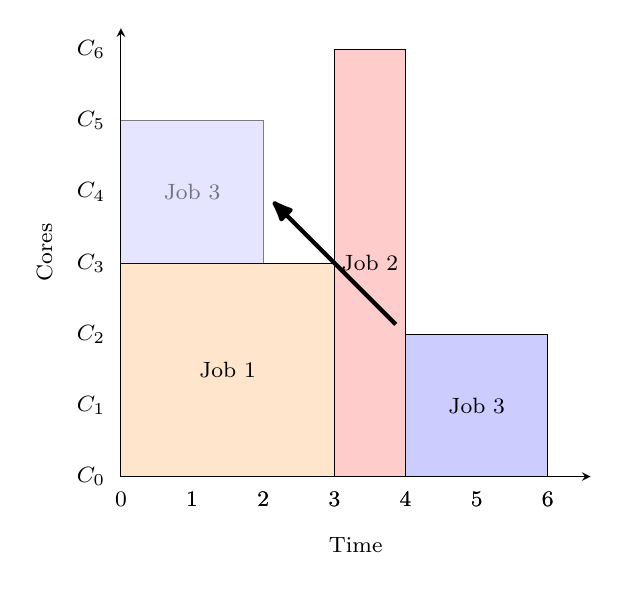
\begin{tikzpicture}\begin{axis}
[ font=\footnotesize,
  ytick style={draw=none},
  xtick style={draw=none},
  unit vector ratio*=1 1 1,
  axis lines = middle,
  enlarge x limits = {value=.1,upper},
  enlarge y limits = {value=.05,upper},
  ylabel={Cores},
  xlabel={Time},
  ylabel near ticks,
  xlabel near ticks,
  const plot,
  stack plots=false,
  area style,
  ytick={1,...,6},
  yticklabels={},  
  xtick={1,...,6},
  extra y ticks={0,1,2,3,4,5,6},
  extra x ticks={0,1,2,3,4,5,6},
  extra y tick style={yticklabel={$C_{\pgfmathprintnumber{\tick}}$}}] 
\addplot[fill=orange!20] coordinates {(0,0) (0,3) (3,3) (3,0)} node at (current path bounding box.center) {Job 1}; 
\addplot[fill=red!20] coordinates {(3,0) (3,6) (4,6) (4,0)} node at (current path bounding box.center) {Job 2}; 
\addplot[fill=blue!20] coordinates {(4,0) (4,2) (6,2) (6,0)} node at (current path bounding box.center) {Job 3};
\addplot[fill=blue!20,opacity=0.5] coordinates {(0,3) (0,5) (2,5) (2,3)} node at (current path bounding box.center) {Job 3};
\node (A) at (4, 2) {};
\node (B) at (2, 4) {};
\draw [->,-{Latex[round]},line width=1.5] (A) edge (B);
\end{axis}\end{tikzpicture}}
\caption{Example of the benefit of conservative backfilling. Job 3 was submitted after job 2 but can be backfilled without delaying the start time of job 2.}
\end{figure}

\todo[inline]{Max: Do we want to say: "When choosing the cores that will be used for a job among the available cores, 
we choose the ones with the lowest index. This allow to optimize the cores utilization and reduce the risk of
creating holes that need backfilling to be used.
Additionaly, when backfilling, the available cores with the smallest next 
start time are chosen in order to fill as much as possible the nodes."}

\section{Working with information from a real workload and cluster\todo[inline]{Max: Another name for this section?}}\label{sec.working}
Actual workloads at HPC resources shared by a great number of users with diverse needs can contain structures
that are non-trivial to replicate in a fully artificial simulated job pattern. We believe that this is especially
true for data-dependent patterns, where a project might launch a burst of jobs using the same file just a few thousand
core hours in length, then be quiet for a long time processing the results, and then launch another such burst.

On the other hand, it would be disruptive to expose a real user community to a wide variety of experimental scheduling strategies.

For this reason, we used logs of historical submitted jobs, in terms of their exact submission time, size, stated runtime, and actual runtime.
Since explicit data dependencies are not encoded in SLURM job specifications, we created an artificial pattern for this. 
\todo[inline]{Carl: Max, please elaborate. Max: Okay, I added a paragraph.}
Each job is carrying an input file.
Let's consider two jobs from the logs of historical submitted jobs: $J_i$ and $J_j$.
They will be attributed a common input file if they match all the following requirements:
\begin{enumerate}
	\item $\core(J_i) = \core(J_j)$ i.e they are requiring the same amount of cores.
	\item $J_i$ and $J_j$ were submitted by the same user.
	\item $J_i$ and $J_j$ were submitted in a 800 seconds timeframe.
\end{enumerate}
Otherwise we consider that $J_i$ and $J_j$ are using distinct input files.

\todo[inline]{Elisabeth: I think we should say Rackham so that readers can checkout the hardware, but perhaps it should be fully blind as a starting point.}
The resource consists of 486 nodes with 20 cores each, with most of them having 128GB of RAM, with some 256GB and 1024GB nodes.

\todo[inline]{Max: I added a paragraph on why all nodes are the same size in our case:}
Having $L$ different nodes sizes raises a new constraint. The model would have
$L$ subsets of nodes, each possibly containing a different number of nodes.
An input file can be too large to be computed on one or multiple of those subsets.
Thus, in addition to the scheduling problem, a load balancing problem arises.
Indeed, the scheduler need to be able to manage each subset of nodes as an independent 
resource that need to avoid starvation while also not being saturated in case of a large
batch of jobs that could be submitted at once and that could only be computed on this node's size.
Consequently, to focus on the issue of data-locality, we use a set of 486 nodes of size 
128 GB and the size of an input file is a multiple of 6.4.
In other words, for each $\file(i) \in \fileset$, $\size(\file(i)) = 6.4 \times n$ with 
$1 \leq n \leq 20$.

The utilization levels are typically high ($>90\%$), but
not fully consistently so. The vast majority of jobs on this resources are single node jobs, even sometimes single core jobs. Run times
could extent to up to 10 days, while some jobs only last a few minutes. We do not claim that this is an ideal job submission strategy,
but rather it is an empirical observation of an actual user community including, but not exclusively consisting of, many subfields of the life sciences with highly data-dependent workflows.

\todo[inline]{Max: Add a paragraph or subsection for this part below?}
Each application scenario is a day on the log's history of the workload.
The way we collect and schedule jobs from the log's history is represented in Figure~\ref{fig.workload}.
\begin{figure*}[tb]
\definecolor{blue}{rgb}{0.38, 0.51, 0.71} %glaucous, 97,130,181, #6182B5
\definecolor{darkblue}{RGB}{17, 42, 60} % 112A3C
\definecolor{red}{RGB}{175, 49, 39} % AF3127
\definecolor{otherred}{RGB}{171,78,78}
\definecolor{orange}{RGB}{237, 126, 75} 
\definecolor{green}{RGB}{104, 174, 89} 
\definecolor{palegreen}{RGB}{197, 184, 104} 
\definecolor{yellow}{RGB}{250, 199, 70} % FAC764
\definecolor{brokenwhite}{RGB}{218, 192, 166} % DAC0A6
\definecolor{brokengrey}{rgb}{0.77, 0.76, 0.82} % {196,194,209}, C4C2D1
\centering\scalebox{1}{
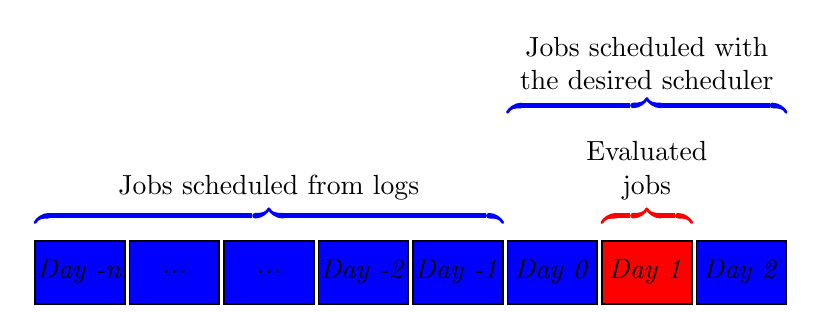
\begin{tikzpicture}[semithick, > = {Stealth[scale=1.25]}, shorten > = 1pt,]
    \def\x{1}\def\y{1}
    \draw[color=black, fill=blue] (1.2*1*\x+0.03, 0.7) rectangle (1.2*2*\x-0.03, -0.1) node[midway] {\textit{Day -n}}; 
    \draw[color=black, fill=blue] (1.2*2*\x+0.03, 0.7) rectangle (1.2*3*\x-0.03, -0.1) node[midway] {\textit{...}}; 
    \draw[color=black, fill=blue] (1.2*3*\x+0.03, 0.7) rectangle (1.2*4*\x-0.03, -0.1) node[midway] {\textit{...}}; 
    \draw[color=black, fill=blue] (1.2*4*\x+0.03, 0.7) rectangle (1.2*5*\x-0.03, -0.1) node[midway] {\textit{Day -2}}; 
    \draw[color=black, fill=blue] (1.2*5*\x+0.03, 0.7) rectangle (1.2*6*\x-0.03, -0.1) node[midway] {\textit{Day -1}}; 
    \draw[color=black, fill=blue] (1.2*6*\x+0.03, 0.7) rectangle (1.2*7*\x-0.03, -0.1) node[midway] {\textit{Day 0}}; 
    \draw[color=black, fill=red] (1.2*7*\x+0.03, 0.7) rectangle (1.2*8*\x-0.03, -0.1) node[midway] {\textit{Day 1}}; 
    \draw[color=black, fill=blue] (1.2*8*\x+0.03, 0.7) rectangle (1.2*9*\x-0.03, -0.1) node[midway] {\textit{Day 2}}; 
    %~ \draw[color=black, fill=blue] (1.2*4*\x+0.03, 0.7) rectangle (1.2*5*\x-0.03, -0.1) node[midway] {Day 3}; 
    %~ \draw[color=black, fill=blue] (1.2*5*\x+0.03, 0.7) rectangle (1.2*6*\x-0.03, -0.1) node[midway] {Day 4}; 
    %~ \draw[color=black, fill=blue] (1.2*6*\x+0.03, 0.7) rectangle (1.2*7*\x-0.03, -0.1) node[midway] {Day 5}; 
    %~ \draw[color=black, fill=blue] (1.2*7*\x+0.03, 0.7) rectangle (1.2*8*\x-0.03, -0.1) node[midway] {Day 6}; 
    %~ \draw[color=black, fill=blue] (1.2*8*\x+0.03, 0.7) rectangle (1.2*9*\x-0.03, -0.1) node[midway] {Day 7}; 
    %~ \draw[color=black, fill=blue] (1.2*9*\x+0.03, 0.7) rectangle (1.2*10*\x-0.03, -0.1) node[midway] {Day 8}; 
    %~ \draw[color=black, fill=blue] (1.2*10*\x+0.03, 0.7) rectangle (1.2*11*\x-0.03, -0.1) node[midway] {Day 9}; 
    %~ \draw[color=black, fill=blue] (1.2*11*\x+0.03, 0.7) rectangle (1.2*12*\x-0.03, -0.1) node[midway] {Day 10}; 
    \draw [pen colour={blue},decorate,line width=2pt,decoration = {calligraphic brace,raise=-2pt,amplitude=5pt}] (1.2*1*\x+0.03, 1) -- node[pos=0.5,above=2pt,black,align=center]{Jobs scheduled from logs} (1.2*6*\x-0.03, 1);
    \draw [pen colour={blue},decorate,line width=2pt,decoration = {calligraphic brace,raise=-2pt,amplitude=5pt}] (1.2*6*\x+0.03, 2.4) -- node[pos=0.5,above=2pt,black,align=center]{Jobs scheduled with\\the desired scheduler} (1.2*9*\x-0.03, 2.4);
    %~ \draw [pen colour={blue},decorate,line width=2pt,decoration = {calligraphic brace,raise=-2pt,amplitude=5pt}] (1.2*4*\x+0.03, 1) -- node[pos=0.5,above=2pt,black,align=center]{Days used to collect all the jobs submitted before \textit{Day 3}} (1.2*12*\x-0.03, 1);
    \draw [pen colour={red},decorate,line width=2pt,decoration = {calligraphic brace,raise=-2pt,amplitude=5pt}] (1.2*7*\x+0.03, 1) -- node[pos=0.5,above=2pt,black,align=center]{Evaluated\\jobs} (1.2*8*\x-0.03, 1);
  \end{tikzpicture}
}
\caption{Methodology followed to schedule and evaluate jobs from a specific day while avoiding edge effects.}\label{fig.workload}
\label{fig.ex}
\end{figure*}
On the real cluster, when a job finishes, it's information
are written in a file corresponding to the day at which the day finished.
This information contains the node that was attributed, the real job's duration, the walltime, 
the number of cores required, the user that submitted the job, the submission time, 
the start and end time.
Our goal is to schedule and evaluate all the jobs submitted on 
\textit{Day 1} in the settings in which they were on the real cluster.
In order to get all the jobs that were submitted on \textit{Day 1}, we need to
look into the logs of days 1 to 10. Indeed, most jobs do not last for more than 10 days,
thus we should cover the vast majority of jobs that were actually submitted on 
\textit{Day 1}.
With this process, we also gather jobs that were started on \textit{Day 0} and \textit{Day 2}. 
Jobs of \textit{Day 1} are respectively preceded and succeeded with jobs from \textit{Day 0}
and \textit{Day 2} in order to place \textit{Day 1} in its "real environment",
i.e. in the situation in which it was on the real cluster, with jobs submitted
before and after, but also to avoid any side effect.
Jobs from \textit{Day -1, -2, ..., -n} are jobs that were submitted before \textit{Day 0} and that are still running at the beginning of \textit{Day 0}.
We use the information from the log's history to start these jobs on the nodes
were they really were scheduled and at the times at which they were started.
This allows us to exactly replicate the state of the cluster on this day before starting
to schedule jobs from \textit{Day 0}.
To summarize, before \textit{Day 0}, jobs are placed on the cluster
following the log's history. Starting from \textit{Day 0} we 
use one of our scheduler and only evaluate jobs submitted on \textit{Day 1}
to avoid any side effect.


\section{Performance evaluation and analysis}\label{sec.evaluations}

We present below the results of experimental evaluations conducted 
on 44 days extracted from logs of historical submitted jobs.

\subsection{Settings}
\todo[inline]{put this somewhere/explain:
We consider that these jobs are dedicated to processing their input
file. Hence, the larger the input file, the more cores the job
requests, such that the file occupies a fraction of the memory
proportional to the number of cores allocated to the job. A job with
$k$ cores will be devoted a memory of size $k M/m$. Thus, we consider
that file sizes are multiple of $M/m$. Max: I think it should go in section 5.}

All strategies as well as the two baselines have been implemented on
a simulator that we developed\todo[inline]{Max: Do we need to say more here?}.

We measure the obtained performance with the mean
stretch from jobs of \textit{Day 1}.
The stretch of a job is the flow of the job divided
by the flow the job would have gotten if it was scheduled on an empty cluster.
They are denoted respectively $Flow(J_i)$ and $\emptyflow(J_i)$.
%~ To compute the flow of a job: $(\start(J_i) + min(\duration(J_i) + t_k' - t_k, \walltime(J_i)) - \submissiontime(J_i))$

\begin{equation}
Flow(J_i) = \Endtime(J_i) - \submissiontime(J_i)
\end{equation}

\begin{equation}
\emptyflow(J_i) = \duration(J_i) + \frac{\size(\file(J_i))}{\bandwidth}
\end{equation}

The stretch of one job is computed as follows:
\begin{equation}
Stretch_{J_i} = \frac{Flow(J_i)}{\emptyflow(J_i)}
\end{equation}

\todo[inline]{Max: Is it okay here to use the $t_k' - t_k$ notation used in the pseudocodes to get the duration of the load that was required?}
\todo[inline]{Max: Do we need a table to recap the acronyms and strategies or reading the section scheduler is sufficient to know the acronyms?}
\todo[inline]{Max: When I show performance of a particular workload should I show both BF and non BF or only one of those? Do I show one and talk about the other one?}
We also evaluate the total amount of time spent waiting for a file to be available.
Our main competitors on this measures will be FCFS and EFT.

\subsection{An underutilized cluster, LEA issues and the appeal of LEM}

\subsubsection{Results}
\todo[inline]{Max: Maybe use paragraphs instead of subsubsection?}

\begin{figure}[tb]\centering\includegraphics[scale=0.47]{../MBSS/plot/Results_FCFS_Score_Backfill_2022-07-16->2022-07-16_V10000_Mean_Stretch_450_128_32_256_4_1024.pdf}\caption{Average stretch of all jobs evaluated on July 16.}\label{stretch.07-16}\end{figure}
\begin{figure}[tb]\centering\includegraphics[scale=0.47]{../MBSS/plot/Results_FCFS_Score_Backfill_2022-07-16->2022-07-16_V10000_Number_of_data_reuse_450_128_32_256_4_1024.pdf}\caption{Number of evaluated jobs re-using a data on July 16.}\label{reuse.07-16}\end{figure}
\begin{figure}[tb]\centering\includegraphics[scale=0.47]{../MBSS/plot/Results_FCFS_Score_Backfill_2022-07-16->2022-07-16_V10000_Total_waiting_for_a_load_time_and_transfer_time_450_128_32_256_4_1024.pdf}\caption{Amount of time spent waiting for a file to be available on July 16.}\label{load.07-16}\end{figure}

Figure~\ref{stretch.07-16} shows us the mean stretch on all jobs.
The horizontal black dotted line correspond to a stretch of 1.
It's the stretch obtained if all the jobs 
are scheduled on an empty cluster.
Thus, it means that the waiting time of a job was exactly
the time it took to load the input file.
FCFS, EFT, LEO and LEM have mean stretches close to 1.
EFT, LEO and LEM have a small benefit over FCFS thanks to the file re-use.
LEA is 20\% slower.

Figure~\ref{reuse.07-16} and Figure~\ref{load.07-16}
both gives us similar information. The first one 
shows the number of jobs that re-used a file.
Meaning that the file load was either nul or 
the job was scheduled with another job loading the same file
at the same time. The gray background denote the total
number of jobs that re-used or not a file.
The second figure plot the total amount of time spent 
waiting for a file to be ready before starting the computation.
On both of these figures, LEA is the outlier:
it re-uses input files for more jobs and consequently the total time spent waiting for a load is lower.

\subsubsection{Understanding LEA's poor performance}

\begin{figure}[H]\centering\includegraphics[scale=0.47]{../MBSS/plot/Cluster_usage/2022-07-16->2022-07-16_V10000_Fcfs_Used_nodes_Reduced_450_128_32_256_4_1024_core_by_core.pdf}\caption{Visualization of the utilization rate of the cluster on the workload of July the 16th with FCFS.}\label{07_16_cluster_usage_fcfs}\end{figure}
\begin{figure}[H]\centering\includegraphics[scale=0.47]{../MBSS/plot/Cluster_usage/2022-07-16->2022-07-16_V10000_Fcfs_with_a_score_x500_x1_x0_x0_Used_nodes_Reduced_450_128_32_256_4_1024_core_by_core.pdf}\caption{Visualization of the utilization rate of the cluster on the workload of July the 16th with LEA.}\label{07_16_cluster_usage_lea}\end{figure}
\begin{figure}[tb]\begin{subfigure}[b]{0.49\linewidth}\centering\includegraphics[width=1\linewidth]{../MBSS/plot/Stretch_times/Stretch_times_FCFS_LEA_2022-07-16->2022-07-16_V10000_450_128_32_256_4_1024.pdf}\caption{With LEA.}\label{07_16_fcfs_vs_lea}\end{subfigure}
\begin{subfigure}[b]{0.49\linewidth}\centering\includegraphics[width=1\linewidth]{../MBSS/plot/Stretch_times/Stretch_times_FCFS_LEM_2022-07-16->2022-07-16_V10000_450_128_32_256_4_1024.pdf}\caption{With LEM.}\label{07_16_fcfs_vs_lem}\end{subfigure}\caption{Stretch times of each job compared to FCFS on the workload of July the 16th.}\end{figure}

To understand the issues LEA encounter on this workload, we need to study the cluster's usage over time.
Figure~\ref{07_16_cluster_usage_fcfs} shows us a visual representation of 
our cluster's usage over time when using FCFS.
The Y axis represents the number of requested cores either running on a node (lower half) or in the queue of jobs waiting to be executed (top half).
The solid blue line shows the number of cores from all jobs.
%~ The dashed blue line shows the additional number of cores that would be needed
%~ to run all the jobs in the queue at a given time (this would thus be the number
%~ of used cores if all the jobs where running in parallel).
The red lines show the jobs in both categories that have their submission
time within our evaluation window, in other words they are sub-parts of the blue line
that we evaluate.

By looking at the top half of Figure~\ref{07_16_cluster_usage_fcfs}
we understand that the job's queue is empty most of the time. In this situation, FCFS is very efficient. Indeed, choosing the earliest available node will in most cases choose a node that can immediately start the job, explaining the mean stretch close to one on Figure~\ref{stretch.07-16}.
LEO is a strategy that uses the earliest available time of a node $t_k$ to decide if it should compute a score like LEA or 
or weigh the transfer time and $t_k$ in the 
equally. This allows LEO to have a behavior close to FCFS or EFT on underused clusters.
Similarly, LEM switches between EFT and LEA depending on the clusters usage, it thus behave similarly to EFT on this particular workload.
On the contrary, LEA favours data re-use over an early start time for a job.
On an underused cluster it will increase startvation.
We can notice this when looking at
Figure~\ref{07_16_cluster_usage_lea}. It shows the custer usage when using LEA on this workload. We can notice that it uses fewer cores, notably before the first vertical orange dotted line. 
This translates into a larger queue of jobs that you can see on the top half of the figure. Jobs in this queue are jobs that already have a valid copy of their file loaded on a node. The benefit of scheduling 
these jobs immediately on another node and loading the file appears inferior to waiting for a file re-use for LEA and thus create this queue of jobs that does not exist for FCFS. 
The consequence in term of stretch is immediately noticeable on Figure~\ref{07_16_fcfs_vs_lea}. This visualization shows the stretch's speed-up of each job compared to FCFS. The size of a circle is proportional to the job duration. On the workload of July 16, we can observe columns of jobs submitted at the same time and using the same file, meaning LEA was waiting to re-use the file to start the jobs, leading in a larger queue time when other nodes are available.

\subsection{An almost saturated cluster, the weakness of LEM and the resilience of LEO}

We saw in the last section the benefit of using LEO or LEM over LEA. Here we evaluate our strategies on an almost saturated cluster that underline the weakness of LEM.

\subsubsection{Results}

\begin{figure}[tb]\centering\includegraphics[scale=0.47]{../MBSS/plot/Results_FCFS_Score_Backfill_2022-09-09->2022-09-09_V10000_Mean_Stretch_450_128_32_256_4_1024.pdf}\caption{Average stretch of all jobs evaluated on September 09.}
\label{stretch.09-09}\end{figure}
\begin{figure}[tb]\centering\includegraphics[scale=0.47]{../MBSS/plot/Results_FCFS_Score_Backfill_2022-09-09->2022-09-09_V10000_Total_waiting_for_a_load_time_and_transfer_time_450_128_32_256_4_1024.pdf}\caption{Amount of time spent waiting for a file to be available on September 09.}
\label{load.09-09}\end{figure}

Despite greatly reducing the amount of file transfers as can be seen on Figure~\ref{load.09-09}, LEA and LEM
do not manage to beat FCFS in terms of stretch (see Figure~\ref{stretch.09-09}). LEO has a slightly better stretch.
The performances of LEA are understanble as we saw that it does not perform on underused cluster, but what about LEM?

\subsubsection{A pathological scenario of LEM}

\begin{figure}[tb]
\begin{subfigure}[b]{0.49\linewidth}\centering\includegraphics[width=1\linewidth]{../MBSS/plot/Cluster_usage/2022-09-09->2022-09-09_V10000_Fcfs_Used_nodes_Reduced_450_128_32_256_4_1024_core_by_core.pdf}\caption{With FCFS.}\label{cluster_09-09_fcfs}\end{subfigure}
\begin{subfigure}[b]{0.49\linewidth}\centering\includegraphics[width=1\linewidth]{../MBSS/plot/Cluster_usage/2022-09-09->2022-09-09_V10000_Fcfs_with_a_score_mixed_strategy_x500_x1_x0_x0_Used_nodes_Reduced_450_128_32_256_4_1024_core_by_core.pdf}\caption{With LEM.}\label{cluster_09-09_lem}
\end{subfigure}
\caption{Visualization of the utilization rate of the cluster on the workload of September the 09th.\todo[inline]{Max: Is it readable to have this two figs side by side?}}\end{figure}

The workload of September the 9th, managed by FCFS (see Figure~\ref{cluster_09-09_fcfs}) results in a cluster that alternates between full utilization and an approximately 80\% utilization rate. Thus the queue of requested cores alternates between a few thousands and 0.
Figure~\ref{cluster_09-09_lem} represent the same experiment with LEM. We can see that the queue of requested cores never hits 0. LEM is thus less efficient at filling the cluster in this case, resulting in a worse mean stretch.
In this case, the occupation rate is just above 80\% but not fully 100\%, thus LEM stays on the same strategy as LEA. And as we saw in the last section, it's a sub-optimal heuristics when the cluster is not fully saturated.

\subsection{A saturated cluster, the great benefits of LEA and LEM}\label{sec.03-26}

\begin{figure}[tb]\centering\includegraphics[scale=0.47]{../MBSS/plot/Results_FCFS_Score_Backfill_2022-03-26->2022-03-26_V10000_Mean_Stretch_450_128_32_256_4_1024.pdf}\caption{Average stretch of all jobs evaluated on March 26.}
\label{stretch.03-26}\end{figure}
\begin{figure}[tb]\centering\includegraphics[scale=0.47]{../MBSS/plot/Results_FCFS_Score_Backfill_2022-03-26->2022-03-26_V10000_Number_of_data_reuse_450_128_32_256_4_1024.pdf}\caption{Number of evaluated jobs re-using a data on March 26.}\label{reuse.03-26}\end{figure}
\begin{figure}[H]\centering\includegraphics[scale=0.47]{../MBSS/plot/Cluster_usage/2022-03-26->2022-03-26_V10000_Fcfs_Used_nodes_Reduced_450_128_32_256_4_1024_core_by_core.pdf}\caption{Visualization of the utilization rate of the cluster on the workload of March the 26th with FCFS.}
\label{cluster_usage.03-26_fcfs}\end{figure}
\begin{figure}[H]\centering\includegraphics[scale=0.47]{../MBSS/plot/Stretch_times/Stretch_times_FCFS_LEM_2022-03-26->2022-03-26_V10000_450_128_32_256_4_1024.pdf}\caption{Stretch times of each job of LEM compared to FCFS on the workload of March the 26th.}
\label{vs_fcfs_lem_03-26}\end{figure}

This workload saturate the cluster with FCFS. Indeed, 
as we can see of Figure~\ref{cluster_usage.03-26_fcfs}, the queue of requested cores is several thousand for the whole duration of the evaluated day.
In this situation, re-using files has a significant impact
on the queue times. This is confirmed by both Figures~\ref{stretch.03-26} and \ref{reuse.03-26}: more data locality is 
associated with a smaller stretch. On a saturated vcluster, when the cluster makes a decision, not filling all the cores with the first job of the queue is not crucial.
It's more beneficial to group jobs using the same file because the queue has enough jobs to fill all the nodes.
Thus, LEA's strategy, also found in LEM, allows to gratly reduce the mean stretch. We can observe this, job by job, on Figure~\ref{vs_fcfs_lem_03-26}.

\todo[inline]{Max: Maybe show a gantt chart?}

\subsection{A cluster saturated with small jobs, the best case scenario for LEA and LEM}\label{sec.08-16}

\begin{figure}[tb]\centering\includegraphics[scale=0.47]{../MBSS/plot/Results_FCFS_Score_Backfill_2022-08-16->2022-08-16_V10000_Mean_Stretch_450_128_32_256_4_1024.pdf}\caption{Average stretch of all jobs evaluated on August 16.}
\label{stretch.08-16}\end{figure}
\begin{figure}[H]\centering\includegraphics[scale=0.47]{../MBSS/plot/Cluster_usage/2022-08-16->2022-08-16_V10000_Fcfs_Used_nodes_Reduced_450_128_32_256_4_1024_core_by_core.pdf}\caption{Visualization of the utilization rate of the cluster on the workload of August 16 with FCFS.}
\label{cluster_usage.08-16_fcfs}\end{figure}
\begin{figure}[H]\centering\includegraphics[scale=0.47]{../MBSS/plot/Cluster_usage/2022-08-16->2022-08-16_V10000_Fcfs_with_a_score_mixed_strategy_x500_x1_x0_x0_Used_nodes_Reduced_450_128_32_256_4_1024_core_by_core.pdf}\caption{Visualization of the utilization rate of the cluster on the workload of August 16 with LEM.}
\label{cluster_usage.08-16_lem}\end{figure}

From Figure~\ref{stretch.08-16}, we observe that LEA has a stretch 33 times lower than
it's competitor. LEM is almost 7 times lower. This drastic diminution is explained
by two particularities of this workload. Firstly, it's a workload that heavily saturate the cluster (as can be seen on Figure~\ref{cluster_usage.08-16_fcfs}, note that the y axis of the top half is modified here to denote the large amount of requested cores compared to the total amount of cores).
Secondly, it's a workload largely composed of jobs that are short and using less than five cores.
Reducing the transfer times of small jobs has a much greater effect on the stretch.
\todo[inline]{Max: explain more}

\todo[inline]{Max: Compute the number of small jobs of this workload and compare it with the average ?}

\subsection{Final results on 44 different evaluated workloads}

\begin{figure}[tb]\centering\includegraphics[scale=0.47]{../MBSS/plot/BF_AND_NON_BF_Results_FCFS_Score_Backfill_2022-01-28->2022-01-28_V10000_Mean_Stretch_450_128_32_256_4_1024.pdf}\caption{Average stretch of all jobs evaluated on January 28.}\label{stretch.01-28}\end{figure}
\begin{figure}\centering\includegraphics[scale=0.47]{../MBSS/plot/Boxplot/box_plot_mean_stretch_all_workloads.pdf}\caption{Mean stretch's speed-up from FCFS on all evaluated workloads. The whiskers are the octiles. The solid green line represent the median and the dashed one the mean.}\label{boxplot.all}\end{figure}
\begin{figure}\centering\includegraphics[scale=0.47]{../MBSS/plot/Boxplot/box_plot_mean_stretch_all_workloads_bf.pdf}\caption{Mean stretch's speed-up from FCFS-BF on all evaluated workloads.}\label{boxplot.all_bf}\end{figure}
\begin{figure}\centering\includegraphics[scale=0.47]{../MBSS/plot/ECDF/ecdf_mean_stretch_all_workloads.pdf}\caption{Empirical distribution function of the mean stretch's speed-up from FCFS on all evaluated workloads.}\label{ecdf}\end{figure}

We can read on Figure~\ref{boxplot.all} a boxplot showing the aggregated
results of mean stretch's speed-up compared to FCFS over all evaluated workloads.
50\% of the results are in the box.
The whiskers delimit to the octiles, thus 75\% of the results are contained
within the whiskers. It also means that between the lower side of the box and the maximum value,
we find 75\% of the results (and similarly between the upper side of the box and the minimum value).
The solid red lines delimit the median while the dashed one shows the mean. 
Each white circle are outliers of which the speed-up is in the first or last octile.
As in the previous results, we observe that EFT does not bring any real improvement compared to FCFS.
\todo[inline]{Max: Should we draw on the whiskers the repartition (12.5,12.5,25,25,12.5,12.5)?}
For LEA, LEO and LEM, the median are respectively 1.12, 1.03 and 1.13. 
However the mean values are much higher at 2.26, 1.21 and 1.76.
We can explain this huge increase from the good performance of LEA's strategy on locality
on heavily saturated clusters (see section~\ref{sec.03-26} and \ref{sec.08-16}).
In these cases, the mean stretch of LEA or LEM are much smaller than those of FCFS or EFT.
For LEO, 87,5\% of the results are above a speed-up of 1.

Figure~\ref{boxplot.all_bf} shows the results but with the backfilling version of our schedulers and compared to FCFS-BF over all workloads.


From the same data shown Figure~\ref{boxplot.all}, we plot an empirical distribution function on Figure~\ref{ecdf}.
EFT's low variance is clearly visible in the sudden jump in probability around a speed-up of 1.
It is interesting to note that for LEA and LEM, 20\% of the results have a speed up of more than 2.5.
In addition, the switch between EFT and LEA for LEM clearly reduces
performance's losses before the black line for LEM.
We can also learn from this figure that LEO is in every respect a better version of EFT.
Indeed, it does not have a higher probability before 1 and after, has significantly more
results at after an 1.2 speed-up.

\todo[inline]{Max: -Talk about perfs, jump in ECDF, outliers, mean and median. ECDF and ECDF BF are similar. Say that we logically gain more on FCFS than FCFS BF, thus the results are like that. 01-28 is a good example to talk about it and show on the same plot with and without backfilling.}

\todo[inline]{LM: should we say somewhere that we tested with stronger data persistence and it did not really helps?}

\section{Conclusion}\label{sec.conclusion}

\todo[inline]{Max: - Fairness - Advance reservation - Tune LEM - Improve locality of LEO}

\bibliographystyle{IEEEtran}
\bibliography{ref.bib}
\end{document}
